\documentclass{isprs}
\usepackage{subfigure}
\usepackage{setspace}
\usepackage{geometry}
\usepackage{epstopdf}
\usepackage{booktabs}
\usepackage{enumitem}
\usepackage{url}


\geometry{a4paper, top=25mm, left=20mm, right=20mm, bottom=25mm, headsep=10mm, footskip=12mm}
%\usepackage{enumitem}

%\usepackage{isprs}
%\usepackage[perpage,para,symbol*]{footmisc}

%\renewcommand*{\thefootnote}{\fnsymbol{footnote}}



\begin{document}
\title{Open source approach to urban growth simulation}

\author{
A. Petrasova\textsuperscript{a,b,}\thanks{Corresponding author}\,,
V. Petras\textsuperscript{a,b},
D. Van Berkel\textsuperscript{a},
B. A. Harmon\textsuperscript{a,d},
H. Mitasova\textsuperscript{a,b},
R. K. Meentemeyer\textsuperscript{a,c}
}

\address
{
\textsuperscript{a }Center for Geospatial Analytics, North Carolina State University, USA - dbvanber@ncsu.edu\\
\textsuperscript{b }Department of Marine, Earth, and Atmospheric Sciences, North Carolina State University, USA - (vpetras, akratoc, hmitaso)@ncsu.edu\\
\textsuperscript{c }Department of Forestry and Environmental Resources, North Carolina State University, USA - rkmeente@ncsu.edu\\
\textsuperscript{d }Department of Landscape Architecture, North Carolina State University, USA - baharmon@ncsu.edu\\

}

% \commission{VI, }{VI} %This field is optional.
% \workinggroup{VI/4} %This field is optional.
\icwg{}

\abstract
{
Spatial patterns of land use change due to urbanization and its impact on the landscape
are the subject of ongoing research. Urban growth scenario simulation is a powerful tool
for exploring these impacts and empowering planners to make informed decisions. 
We present FUTURES (FUTure Urban -- Regional Environment Simulation) -- a patch-based,
stochastic, multi-level land change modeling framework as a case showing how
what was once a
closed and inaccessible model benefited from integration with open source GIS.
We will describe our motivation for releasing this project as open source
and the advantages of integrating it with GRASS GIS, a free, libre and open source GIS
and research platform for the geospatial domain.  
GRASS GIS provides efficient libraries for FUTURES model development
as well as standard GIS tools and graphical user interface for model users.  
Releasing FUTURES as a GRASS GIS add-on simplifies the distribution of FUTURES
across all main operating systems and ensures the maintainability of our project in the future.
We will describe FUTURES integration into GRASS GIS and demonstrate its usage
on a case study in Asheville, North Carolina.
The developed dataset and tutorial for this case study
enable researchers to experiment with the model, explore its potential or even
modify the model for their applications.
\vspace{4pt}}

\keywords{GRASS GIS, FUTURES, urbanization, land change, open science, simulation}

\maketitle


\newcommand{\normalniradky}{%
\renewcommand{\baselinestretch}{0.96}%
\selectfont%
}

\newcommand{\roztazeneradky}{%
\renewcommand{\baselinestretch}{0.98}%
\selectfont%
}
\section{INTRODUCTION}\label{INTRODUCTION}
\roztazeneradky
Population growth in cities worldwide drives changes in land use
often negatively impacting the environments in which people live and undermining
the resilience of local ecosystems.
The need to understand the trade-offs urban planners are facing
gave rise to a number of different land change simulation models,
which proved to be powerful tools for exploring
alternative scenarios and their impacts on various aspects of human-environmental systems
\cite{chaudhuri2013sleuth,verburg2002modeling,sohl2007fore,waddell2002urbansim}.
Despite the influence of the spatial structure and connectivity 
of urbanizing landscapes on
biodiversity, water quality, or flood risks \cite{alberti2005effects},
most urban growth models are based on cell-level conversions and 
have not focused on generating realistic spatial structures across scales \cite{jantz2005analysis}.
To bridge the gap between cell- and object-based representation, we developed
FUTURES (FUTure Urban-Regional Environment Simulation), a patch-based, multilevel
modeling framework for simulating the emergence of landscape spatial structure
in urbanizing regions \cite{Meentemeyer2012}.
%
The FUTURES model was successfully applied in several cases 
including a study of land development dynamics in the rapidly
expanding metro\-po\-litan region of Charlotte, North Carolina \cite{Meentemeyer2012} and an analysis of the impacts
of urbanization on natural resources under different conservation strategies \cite{Dorning2015}.
Most recently, FUTURES was coupled with ecosystem services models to examine the impacts of projected urbanization and urban pattern on several
ecosystem services and their trade-offs \cite{doug2016,Brian2016}.


In order to study the complex interactions between human and natural systems,
interdisciplinary researchers are coupling
existing simulation models.
Land change modeling plays often a crucial role in these coupled models.
Previous case studies with FUTURES have demonstrated 
that the model can be applied to a wide range of cases with different study systems and aims.
%
The initial implementation of model, however, was a prototype that was not ready
to be shared
with scientific community. 
%
The model accumulated too much ``technical depth'' \cite{easterbrook2014open} during its initial development, 
making it difficult to add new features or run the simulation at larger scales.
%
In order to continue adding new capabilities to FUTURES and to promote
its usage 
both inside and outside of 
the land use community,
we decided to revise the implementation of the FUTURES model 
and develop a new version which would be (a) more efficient and scalable, 
(b) as easy to use as possible for a wider audience and (c)
fully open source and maintainable in the long run.
To achieve these goals we 
decided that instead of keeping FUTURES as a standalone application,
we would take advantage of existing geospatial software and integrate FUTURES
into open source GRASS GIS \cite{Neteler08}.
By using GRASS GIS' efficient geospatial libraries
we can develop better and higher-level code.
%
Providing open source software to the scientific community entails more than just releasing the actual code -- 
documentation, tutorials, installation
instructions, binaries and support are also needed 
and require considerable effort. % Consider explaining why these things are needed
Without this effort, models cannot be practically used by other researchers.
%
By using GRASS GIS' existing infrastructure we could focus on developing the actual materials
instead of managing our own server infrastructure.

In this article we present a new version of the FUTURES urban growth model that is 
available as the \emph{r.futures} module set from the GRASS GIS add-on repository.
This new version of FUTURES
streamlines data processing, provides opportunities to study urbanization on mega-regional scales, 
and allows for more reproducible research in the land change community. 
We demonstrate this new version of FUTURES with a case study of the Asheville metropolitan area in North Carolina, USA.

\normalniradky
% must be open source to attract users chaudhuri2013sleuth


\section{FUTURES model}
FUTure Urban-Regional Environment Simulation
is a stochastic, patched-based model
for projecting landscape patterns of urban growth \cite{Meentemeyer2012}.
FUTURES has a modular structure consisting of 3 main submodels: DEMAND, POTENTIAL and
PGA (patch-growing algorithm), see Figure \ref{fig:schema}.
Land conversion is driven by projected population demand computed by the DEMAND submodel,
and is spatially defined by a probability surface derived by  the POTENTIAL submodel
from multiple environmental and socio-economic predictors.
The population demand and the effects of land change drivers can vary in space by subregions,
such as jurisdictional units, allowing projections across heterogeneous landscape.
FUTURES main strength lies in realistically modeling the 
spatial structure of urban change by growing patches 
that are
parameterized by size and compactness 
and calibrated using historical data.
For a detailed explanation of FUTURES' components, please refer to Meentemeyer et al. (2013).

\begin{figure}[h!]
 \centering
 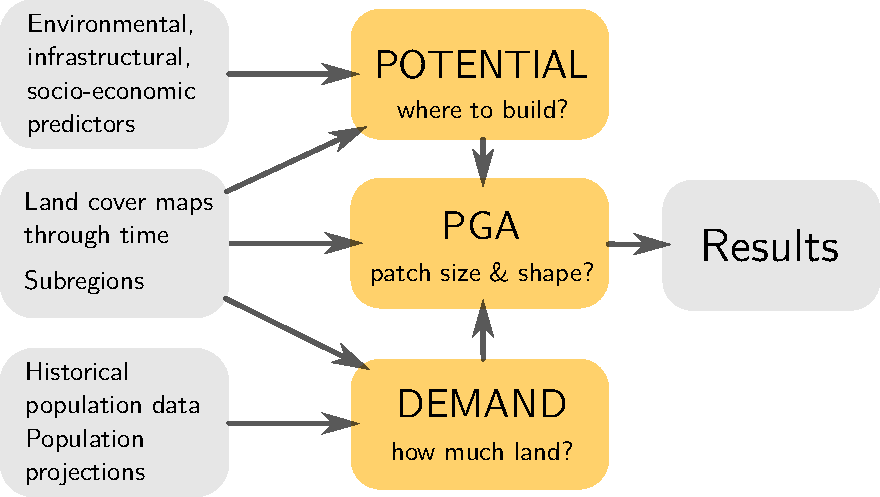
\includegraphics[width=0.9\columnwidth]{./figures/schema.pdf}
 \caption{Simplified schema of FUTURES conceptual model  with inputs and outputs in gray and submodels in yellow}
 \label{fig:schema}
\end{figure}


The original implementation of FUTURES consisted mainly of the patch-growing 
algorithm, a standalone program written in a mixture of C and C++.
The PGA program itself utilized inefficient algorithms and required raster data in ASCII
format as input leading to very slow initialization. % such as linear search in a long sorted list.
The DEMAND submodel was computed in a spreadsheet and POTENTIAL coefficents
were derived using R statistical software. No official
implementation of these submodels existed so each researcher
developed a different workflow. This made it difficult for peers to verify each other's work. 
%
Several scripts for calibrating patch 
characteristics derived with FRAGSTATS \cite{fragstats} existed, however these tools
were written 
in an unnecessarily low-level language
for a specific case 
using the author's directory layout.


When revising the original implementation of FUTURES we identified
several issues which needed to be addressed. 
First, it is important to follow best practices for scientific computing \cite{wilson2014best}
including use of a versioning system, writing documentation and testing.
We also wanted to minimize tasks that had been done manually in order to make the process more efficient and avoid errors 
that are often difficult to detect.
When automating tasks 
we had to compromise between 
the flexibility and simplicity %efficiency
of the workflow.
%
We also focused on making FUTURES scalable 
so that it can run
large scale applications
at a relatively fine spatial resolution.
Finally, we designed FUTURES to be more user-friendly and easy to test so that
anyone can confidently apply it to their research.


\section{INTEGRATION IN GRASS GIS}
GRASS GIS has had a long history as a platform for scientific models \cite{chemin2015grass}.
As an open source GIS used by researchers worldwide and one of the founding projects of OSGeo,
GRASS GIS provides a stable environment for the development of
scientific models 
for studying problems from various domains
including geomorphology, hydrology, planetary science, landscape ecology, hazard mapping, archaeology, renewable energy and transportation.
Thanks to the numerous scientist and developers who have been involved, GRASS GIS today provides a large spectrum of geospatial modules
ranging from basic GIS functionality to highly specialized models.
Most of the specialized tools are not part of standard GRASS GIS installations,
but are easily accessible from the add-on repository.

There were multiple reasons for our decision to integrate FUTURES into GRASS GIS as an add-on. Some of these reasons were specific to FUTURES, but others apply to any spatial, scientific model.
Integrating a model into GIS gives both users and developers
a wide array of standard geospatial tools that simplify the implementation of a model,
and streamline pre- and post-processing and visualization.
%
%From the point of view of the model developer, 
GRASS GIS provides
model developers
a raster library for highly efficient data reading and writing.
This means that FUTURES no longer has to read in ASCII files,
significantly reducing time needed for initialization.
Furthermore, raster data from FUTURES simulations are efficiently compressed.
Despite ever increasing disk space, it is still quite important to reduce the file size, especially for
stochastic spatio-temporal simulations, which typically generate huge datasets.
In order to achieve the best speed performance,
most GRASS GIS functionality is implemented in C.
Because of this, we could easily integrate FUTURES 
code, written in a mix of C and C++, 
without major rewriting. 
For portability reasons we later decided to use the C99 standard.
While C and C++ are the preferred languages for computationally expensive algorithms,
GRASS GIS also supports Python as the primary scripting language. 
This is crucial because FUTURES had many steps of data preparation that we were easily able to automate using Python scripting. 
%
Model developers can appreciate
GRASS GIS' automatic generation of
command line interfaces, Python interfaces and graphical user interfaces (GUI).
%
Simply by defining
options in C or Python modules
we can call the same module from a GUI dialog, a Python script or a Bash script.
A graphical interface makes FUTURES easy to use,
especially for users on the Windows platform. 
A Python or Bash interface, however, is needed for more advanced applications such as running FUTURES in parallel on a high performance computer.
GRASS GIS provides infrastructure for publishing and distributing models to users on all major platforms.
Models and tools in GRASS GIS's Add-on repository\footnote{\url{https://grass.osgeo.org/download/addons/}}
can be easily browsed and installed with their documentation,
relieving researchers 
of the burden of maintaining 
such
infrastructure.

\subsection{Implementation}
We implemented FUTURES as a set of GRASS GIS modules starting with a common prefix \emph{r.futures}:
\begin{itemize}[noitemsep,nolistsep]
 \item \emph{r.futures.demand} extrapolates the area of developed land from population trends and projections.
 \item \emph{r.futures.devpressure} computes the development pressure predictor.
 \item \emph{r.futures.potential} models the development probability surface through multi-level logistic regression.
 \item \emph{r.futures.calib} calibrates patch sizes and shapes.
 \item \emph{r.futures.pga} simulates urban development using the patch growing algorithm.
\end{itemize}
In addition, we implemented the add-on \emph{r.sample.category} needed for the workflow. 
Since its functionality is not specific to FUTURES, 
we kept it separate.
All of these add-ons can be conveniently installed from GRASS GIS using the GUI or command line%
\footnote{\texttt{g.extension r.futures}}. 
Each individual add-on has a manual page accessible both online and offline.
Figure \ref{fig:schemaGRASS} shows FUTURES workflow and the inputs needed for each tool.
In the following sections we describe the developed tools, their functionality and implementation in GRASS GIS.


\begin{figure}[h!]
 \centering
 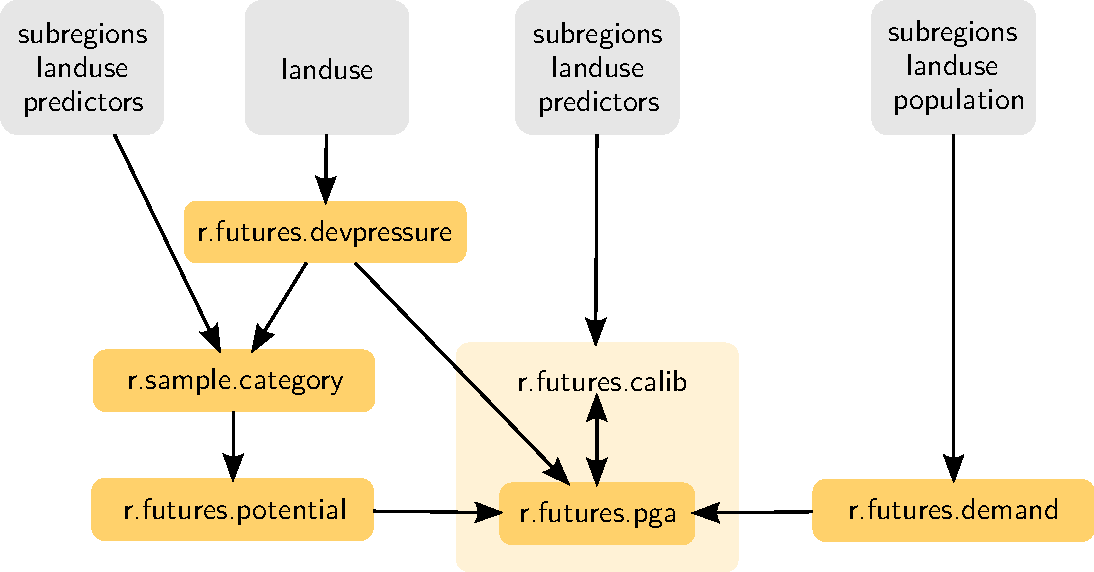
\includegraphics[width=\columnwidth]{./figures/grass_futures_diagram.pdf}
 \caption{Diagram of FUTURES workflow showing how are \emph{r.futures} modules (yellow boxes) chained 
 and what are their input data (grey boxes). As indicated by the light yellow box,
 module \emph{r.futures.calib} calls \emph{r.futures.pga}.}
 \label{fig:schemaGRASS}
\end{figure}


\subsubsection{r.futures.demand}
Based on historical land development and population growth, the DEMAND submodel 
(implemented as \emph{r.futures.demand})
projects the rate of per capita land consumption for each year of the simulation
and each subregion. This Python module uses GRASS GIS Python Scripting Library 
and the NumPy, SciPy and matplotlib 
libraries for scientific computing
to approximate the relation between population and land consumption
with a statistical model described by a linear, logarithmic or exponential curve.
For example, a logarithmic relation means that a growing population requires
less developed land per person over time.
With enough data points, the module
can select the best curve for each subregion based on residuals.
The primary outputs are plain text files with tab-separated values
representing the number of cells to be converted to developed land each year for each subregion.
The module
plots the resulting curves and projected points for each subregion (Figure \ref{fig:demand}) 
so that the results can be visually inspected.
The module \emph{r.futures.demand} provides a fast way to estimate
the land demand given a large number of subregions with diverse population
trends and thus allows us to quickly explore different population scenarios.

\begin{figure}[h!]
 \centering
 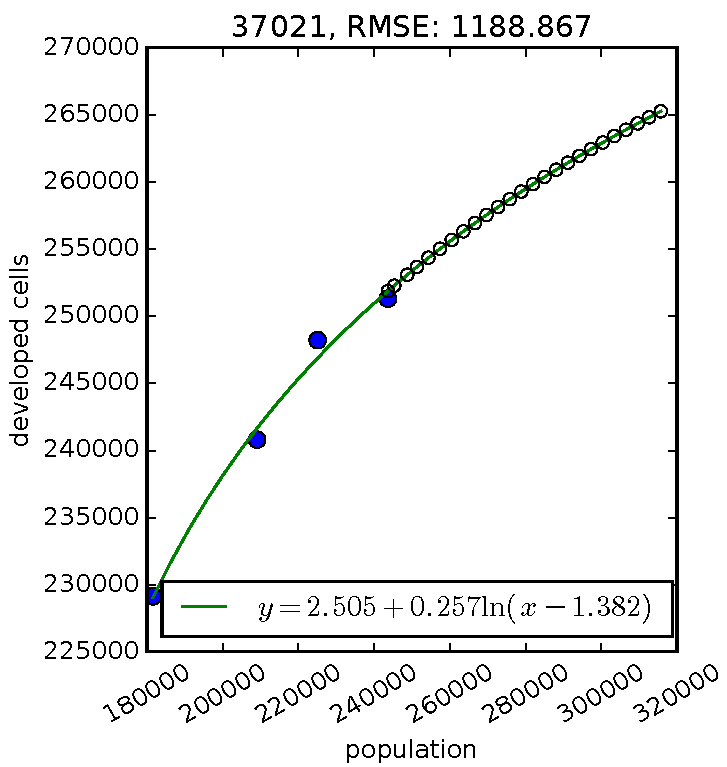
\includegraphics[width=0.4\textwidth]{./figures/plot_demand.pdf}
 \caption{An example of \emph{r.futures.demand} output plot showing
 the logarithmic relation between population and land consumption
 for the county with ID 37021.
 Observed data are showed as blue dots and predicted data as circles.
 }
 \label{fig:demand}
\end{figure}

\subsubsection{r.futures.devpressure}
Development pressure is one of the most
important predictors of where development is likely to happen.
For each cell it is computed as a distance decay function of neighboring
developed cells \cite{Meentemeyer2012}.
Compared to the tool previously used for computing development pressure,
the new Python module \emph{r.futures.devpressure} provides a faster and more efficient 
implementation by taking advantage of the existing GRASS GIS 
module \emph{r.mfilter} written in C for moving window analysis with custom designed matrix filters.
By precomputing the matrix of distances we avoid repeated distance computations
resulting in faster processing. 
Because the new implementation
is less memory intensive 
it can be used for
larger regions than the previous tool. 

\subsubsection{r.futures.potential}
uses multilevel logistic regression  to model development
suitability based on environmental, infrastructural, and socio-economic predictors such as distance to roads or topographic slope.
We randomly sample these predictors and the observed change from undeveloped to developed cells
to estimate the coefficients of the multilevel logistic regression.
The core of this
module is a script in the R language \cite{rstats}, which uses the package lme4 \cite{lme4}
for fitting generalized linear mixed-effects models and the package MuMIn \cite{mumin}
for automatic model selection.
The output file is a plain text file with tab-separated regression coefficients.
This script is wrapped in Python for more seamless processing
and chaining of modules. 
The coupling between R, Python and GRASS GIS
is intentionally very loose to make the workflow possible in the Windows environment
where some of the other, more elegant, options such as
rpy2\footnote{rpy2 is a Python package for using R from Python (\url{http://rpy2.bitbucket.org/})} are complicated to use.
We performed stratified sampling of observed new development and predictors using GRASS GIS add-on \emph{r.sample.category}. 
Although we developed this add-on for urban growth modeling with FUTURES,
its application is much broader. 
In order to encourage its use in other applications we made it a general module rather than making it part of the \emph{r.futures} tool set.

\subsubsection{r.futures.pga}
is the main engine of FUTURES -- it simulates urban growth using inputs from the
DEMAND and POTENTIAL submodels.
The patch growing algorithm (PGA) sto\-chasti\-cally allocates
a seed for new development across the development suitability surface,
challenges the seed by comparing it with a random number between 0 and 1, and
then grows a discrete patch from the seed if it survives \cite{Meentemeyer2012}. 
This process repeats
until the number of converted cells specified by DEMAND is met.
The development pressure predictor and then
the development suitability values are updated based on the newly developed cells.
(The development suitability is computed internally
from predictors and regression coefficients supplied by POTENTIAL.)
We kept the original patch growing algorithm,
but significantly improved its implementation to make it
faster, more memory efficient and simpler to use.
We replaced a custom, undocumented configuration file with a standard module interface
usable from GUI or the command line, and restructured the input and output
parameters and their names so that they are easy for users to understand. 
We used efficient GRASS GIS libraries for reading and writing raster data,
which minimized the time needed to initialize the simulation.
FUTURES now reads rasters in GRASS's native format
instead of ASCII files. 
This decreased the time needed for model initialization from several minutes to several seconds
for a region with tens of millions of cells.
Furthermore, we replaced the static allocation of internal structures with dynamic allocation
and reduced the overall memory requirements 
so that FUTURES could run on large regions with tens or hundreds of counties
as well as smaller areas like our case study.
Finally, through the use of appropriate programming techniques, such as binary search, we significantly increased the
speed of the algorithm.

\subsubsection{r.futures.calib}
We developed a dedicated Python module for calibrating patch sizes and shapes
that runs the module \emph{r.futures.pga}
with different combinations of patch parameters and outputs a table
with scores for each combination of patch parameters.
%
The simulation is run
multiple times for each combination 
to account for the stochasticity of the model.
To speed up the calibration process \emph{r.futures.calib} can take advantage of multiple
computer cores.

\section{CASE STUDY}
To demonstrate how the new FUTURES framework
can be used to simulate urban growth,
we present a case study for 
Asheville metropolitan area located in the Blue Ridge Mountains in the west of North Carolina, USA.
The region consists of five counties with total area of 6,271 km$^2$ and around 477,000 people
based on 2014 population estimates.
It is characterized by rapid population growth around Asheville, the largest city of the region.
New development is constrained by the steep mountainous terrain and large national and state parks.
We simulate urban growth from 2012 to 2030 using publicly available data,
including the USGS's National Land Cover Database (NLCD)  \cite{nlcd2011,nlcd2006,nlcd2001,nlcdretro},
past estimates and future projections of county populations \cite{NCOSBM},
boundaries and roads provided by the United States Census Bureau's database (TIGER)
and a digital elevation model from the National Elevation Dataset (NED) distributed by the USGS.

\begin{figure}[h!]
 \centering
 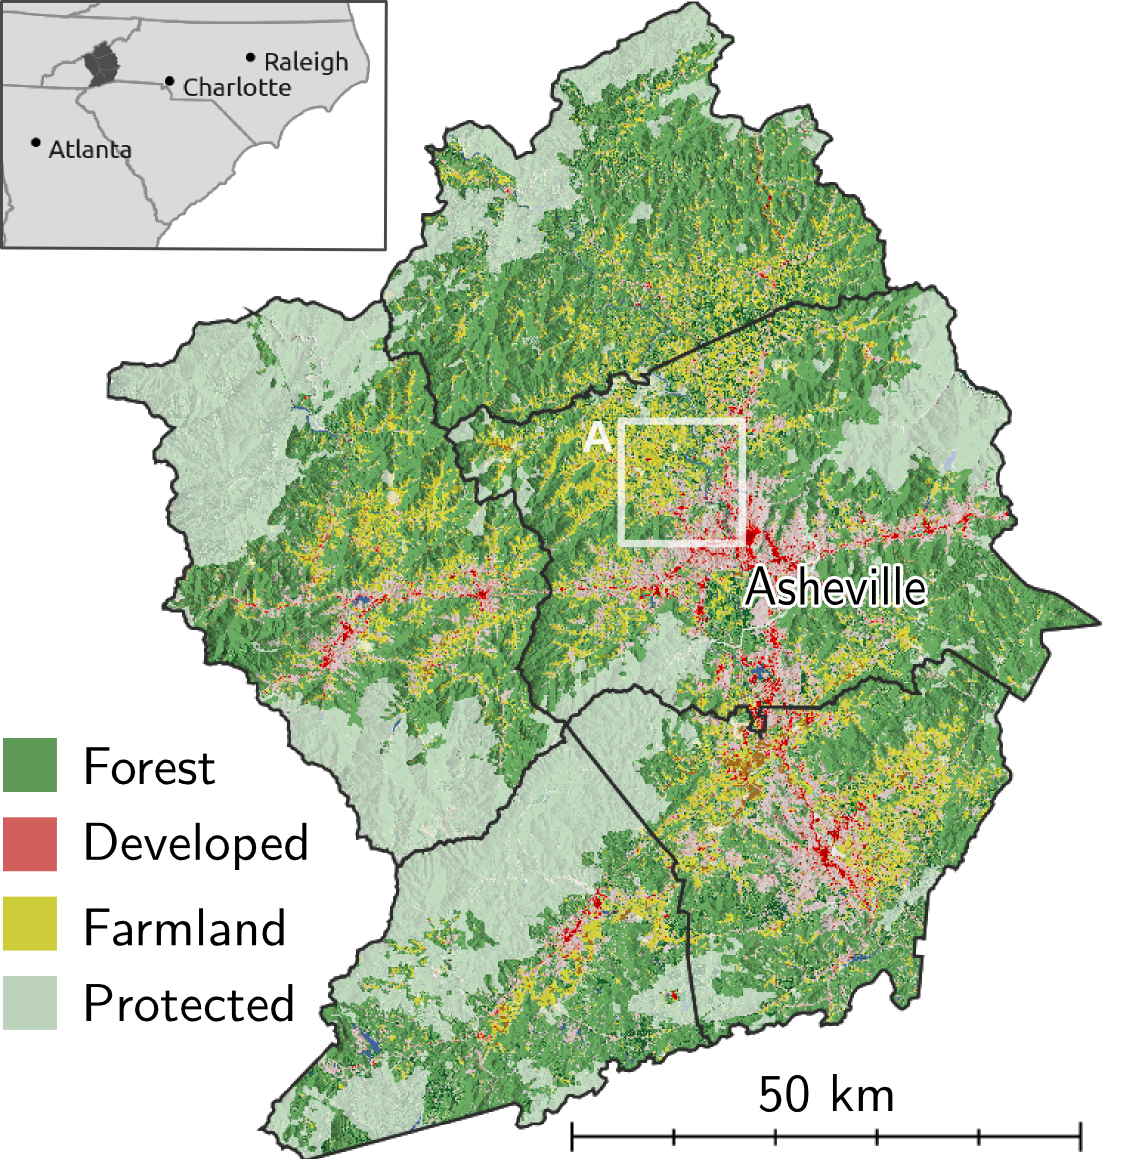
\includegraphics[width=\columnwidth]{./figures/study_area_all.png}
 \caption{2011 land cover \protect\cite{nlcd2011} and protected areas \protect\cite{anderson2011conservation} in the Asheville metropolitan area in the west of North Carolina, USA. Inset A is used in Figure~\ref{fig:results}.}
 \label{fig:study_area}
\end{figure}

\subsection{Approach}
There are several steps required to run the FUTURES simulation:
\begin{itemize}[noitemsep,nolistsep]
 \item Preprocess the data.
 \item Estimate per capita land consumption 
controlling the total area of converted land.
 \item Derive the development suitability statistical model to control where the new development happens.
 \item Calibrate patch size and shape.
 \item Run the urban growth simulation.
\end{itemize}
%(a) preprocess the data,
%(b) estimate per capita land consumption 
%controlling the total area of converted land,
%(c) derive the development suitability statistical model to control where the new development happens,
%(d) calibrate patch size and shape and finally 
%(e) run the urban growth simulation.

\subsubsection{Data preparation}
The core input data for urban growth modeling with FUTURES is a timeseries of land cover maps,
which can be derived by various methods from satellite imagery. 
In this study
we used the 2001, 2006 and 2011 NLCD Land Cover products 
and 1992/2001 Retro\-fit Land Cover Change product to derive a 30-meter binary representation
of developed areas. We excluded national and state parks,
water bodies and wetlands from further analysis. 
We used NLCD products that are available for the contiguous USA 
so that this study and its workflow would be easier to reproduce and apply to other study areas.
We obtained population statistics from the North Carolina Office of State Budget and Management,
which are based on 2000 and 2010 censuses and include past as well as future estimates
of population per county for each year up to 2035. Data for the 5  counties studied
were extracted and formatted as a comma-separated values (CSV) file.

\subsubsection{DEMAND}
We derived the relation between population
and land consumption
from the series of binary rasters of developed areas and
population statistics
to model how much land will be developed
each year of the simulation.
Using the module \emph{r.futures.demand} we explored different curve fitting
methods and derived the per capita land consumption
from period 1992 through 2011, which was characterized by
population growth with decreasing demand for land per person over time.
We expect similarly low rates of per capita land consumption
in the following years because development is restricted by the mountainous terrain and
large protected areas.
Based on RMSE and visual inspection of the plots
created by \emph{r.futures.demand} we
selected either linear or logarithmic relations % ($y = a \ln(x) + c$)
for each county, where the function coefficients were  automatically determined using linear regression and non-linear least squares optimization 
in \emph{r.futures.demand} (Figure \ref{fig:demand}).


\begin{figure*}[tbh]
 \centering
 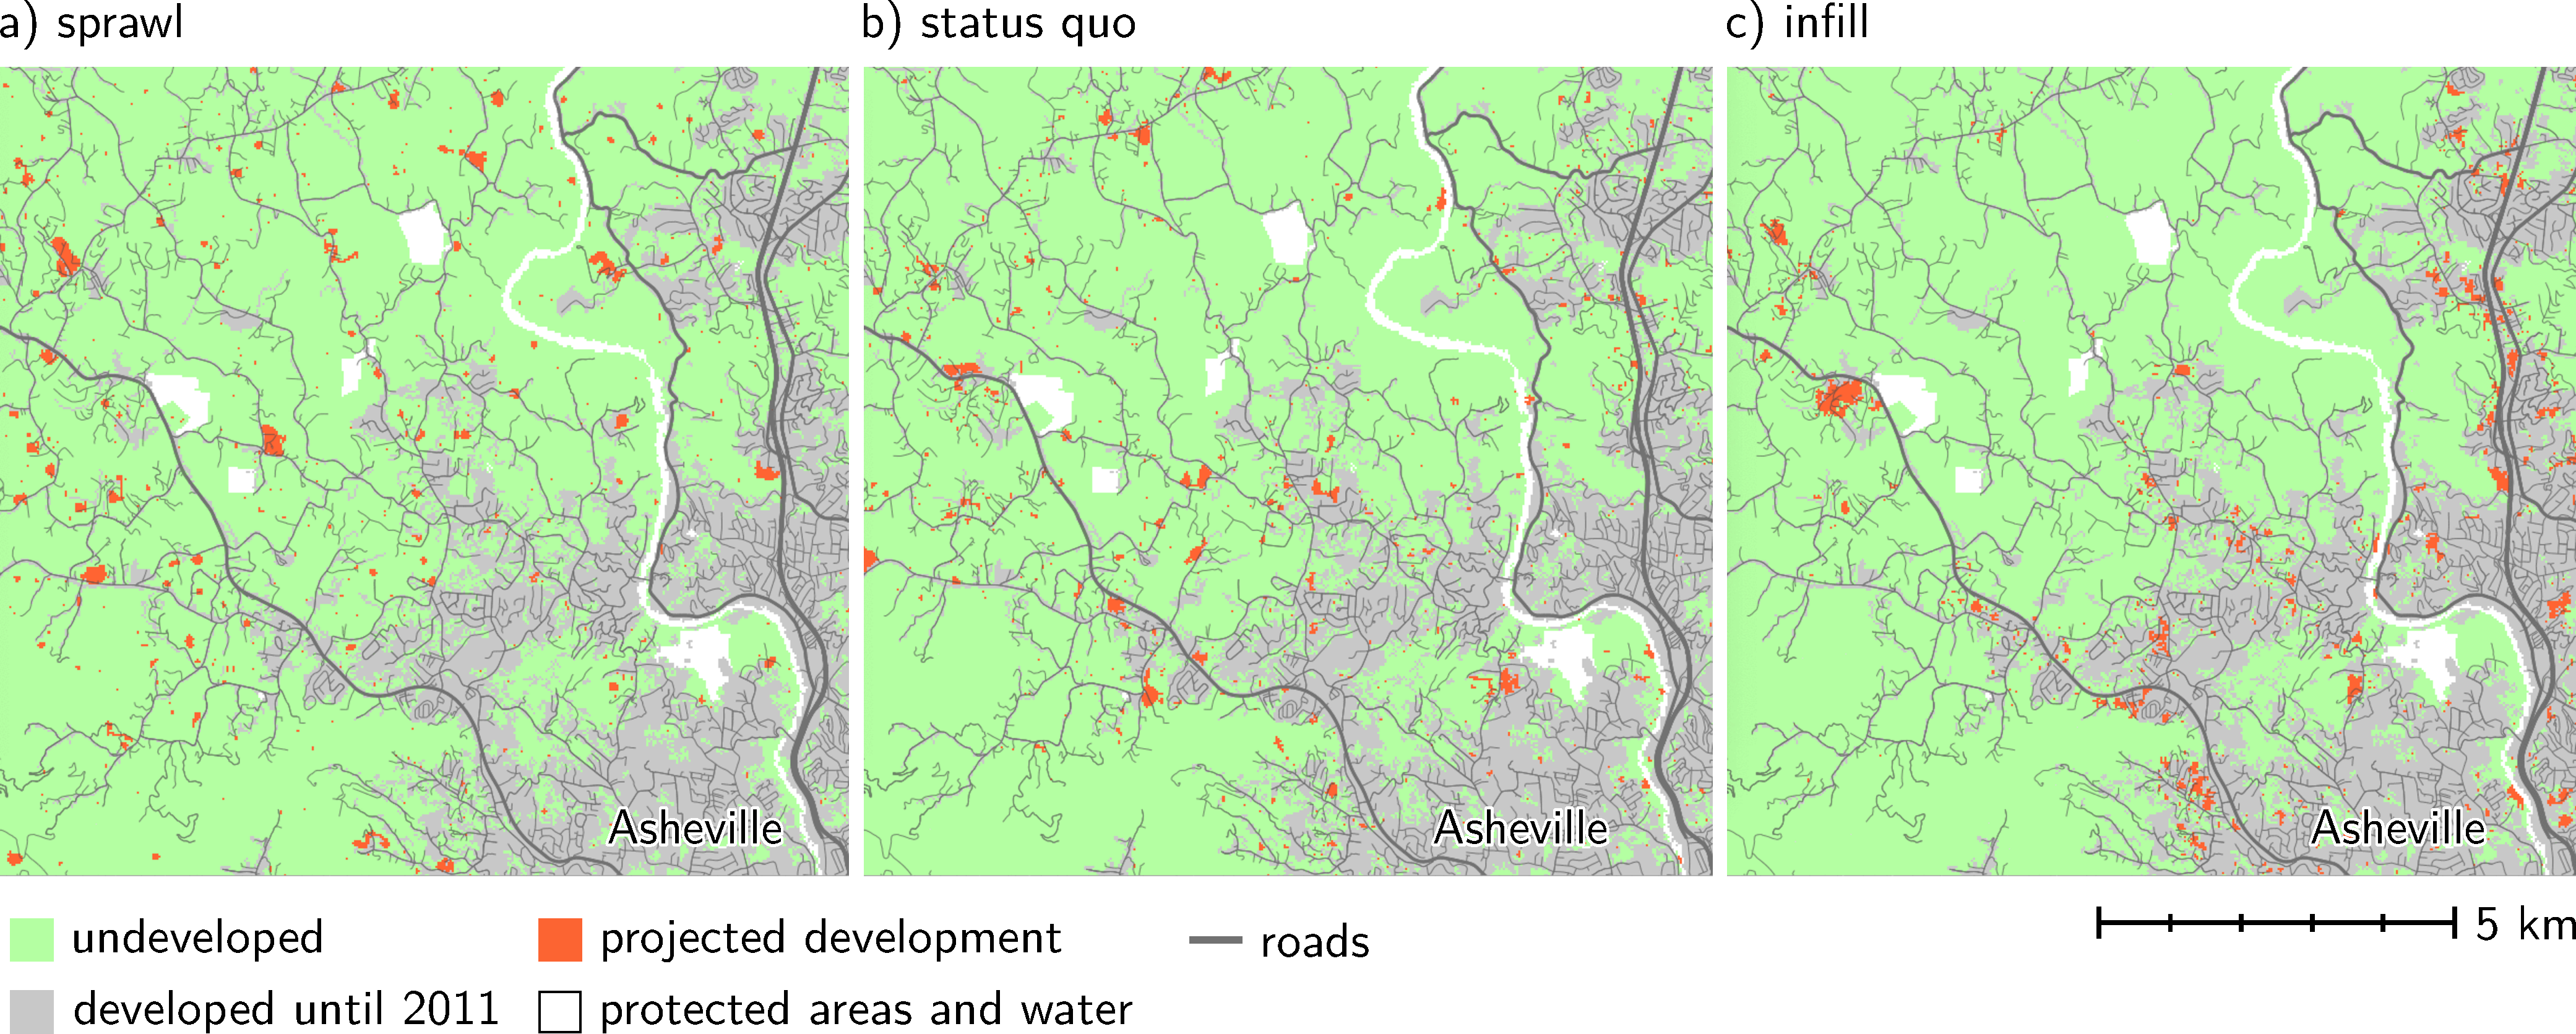
\includegraphics[width=2.0\columnwidth]{./figures/results_maps.pdf}
 \caption{Results of three realizations of multiple stochastic runs with different scenarios.
 Depending on the scenario, simulated development is more diffuse (a) or more compact (c).}
 \label{fig:results}
\end{figure*}

\subsubsection{POTENTIAL}
We used multilevel logistic regression to predict
where new development happens based on
environmental, infrastructural and socio-economic site suitability
predictors. 
Using \emph{r.sample.category} we sampled predictors on 8000 
randomly selected locations and estimated the model coefficients
using the R package lme4 integrated into the module \emph{r.futures.potential}.
The sample points were stratified by the response variable
where new sites developed since 1992 have a value of 1
and sites that are undeveloped in 2011 have a value of 0.
We included counties as the group level indicator
in the multilevel model to account for differences
across jurisdictional boundaries.
From the initial list of hypothesized predictors
(slope, distance to water, protected areas, interchanges,
travel time to cities and towns, forest occurrence and road density)
we identified a set of predictors (Table \ref{tab:predictors})
resulting in a model with the lowest AIC (Akaike information criterion) score.
We verified the robustness of the selected predictors
by repeating the random sampling and model selection process multiple times.
In addition to these predictors, we included also development pressure,
 a special, dynamic predictor that is
 updated during the simulation based on new simulated development to enable positive feedback.
We computed the initial development pressure raster
with \emph{r.futures.devpressure}; its subsequent updates are performed in memory during the simulation.

\begin{table}[htb]
 \centering
\begin{center}
\begin{tabular}{lrr}
\toprule
Predictors & Estimate{\scriptsize *} & Std. Error \\ \midrule
Intercept (varies by county) & -2.593 & 0.269\\
Development pressure & 0.058 & 0.005\\
Road density & 0.118 & 0.007\\
Percentage of forest & -0.013 & 0.002 \\
Distance to protected areas & -0.140 & 0.039\\
Distance to water bodies & -0.148 & 0.022\\
\bottomrule
{\scriptsize * all P-values $<$ 0.001}
\end{tabular}
\end{center}
 \caption{List of selected predictors and estimated coefficients
 for site suitability model}
 \label{tab:predictors}
\end{table}

\subsubsection{Patch calibration}
Prior to running the urban growth simulation implemented in \emph{r.futures.pga}
we calibrated the input patch compactness and size to match
the simulated patterns with the observed patterns from 1992 to 2011.
Since calibration is a time consuming process, we ran the module
\emph{r.futures.calib} for Buncombe county 
and applied the results to the rest of our study region.
We choose Buncombe County which includes the city of Asheville  because it is where most new development will occur.
For each combination of patch parameters we compared the patch characteristics 
averaged from 20 runs of the urban growth simulation with the known patches.
Based on the score we selected patch parameters resulting in high compactness
which is expected for mountainous regions.


\subsubsection{Urban growth simulation}
Having collected all necessary input data, we ran 
\emph{r.futures.pga} with a 1 year time step until 2035 for the entire study region at 30 m resolution.
To account for different future policies regarding new development, we explored
scenarios altering the site suitability to encourage infill or sprawl by changing
\texttt{incentive\_power} parameter of \emph{r.futures.pga}. This value transforms
the probability $p$ a cell is developed to $p^x$ where $x = 1$ represents status quo,
higher values of $x$ result in infill and lower values in sprawl.
In addition to the status quo we simulated scenarios with $x$ equals 0.25, 0.5, 2 and 4.
We repeated each scenario 50 times to account for the model's stochastic behavior.



\subsection{Results}
The resulting development patterns of three realizations of the random runs
are visible in Figure \ref{fig:results}
for the status quo, infill scenario ($x = 4$) and sprawl scenario ($x=0.25$).
The simulated patches realistically mimic the current patches of development in shape and size
and are mostly, but not exclusively adjacent to roads as expected.
Furthermore, we post-processed the results to study how different urban growth policies
influence the loss of forest and agricultural land in the Asheville area
(Figure \ref{fig:results_plot})
by averaging the loss of both land use categories over the 50 runs.
In all scenarios, forest is more affected by future development than farmland.
The extreme case of urban sprawl results in twice as much forest as farmland being developed.
Status quo scenario leads to the smallest difference between the areas converted to forest and farmland.
Interestingly, infill scenario develops the forested area in a similar way as sprawl does, which 
is not surprising considering developed areas are largely surrounded by forest patches.

\begin{figure}[!ht]
 \centering
 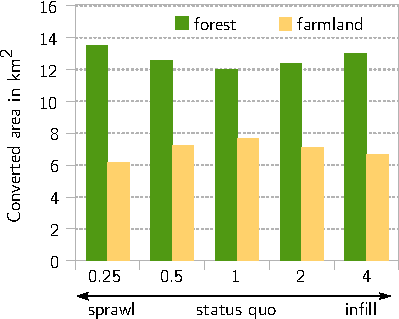
\includegraphics[width=0.9\columnwidth]{./figures/converted_land_new.pdf}
 \caption{Area in km$^2$ of converted land from forest (green) and farmland (yellow) to urban
 differs for urban sprawl and infill scenarios. Numbers $0.25$ to $4$ represent the exponent $x$ which
 transforms development probability $p$ to $p^x$.}
 \label{fig:results_plot}
\end{figure}


Table \ref{tab:benchmark} shows the computational resources
necessary for running this case study and compares 
the time and memory requirements with the original
implementation of FUTURES. Note that
our study area is fairly small (12 million cells)
and when applied to larger regions with more projected development, 
the expected speed gain is even more significant
as we changed the complexity of one of the core algorithms from linear to logarithmic.
Because the individual stochastic runs are independent of each other
this simulation is an
``embarrassingly parallel''  problem \cite{herlihy2012art}
in which the computation can easily be distributed across multiple computer cores.

\begin{table}[htp]
 \centering
\begin{center}
\begin{tabular}{lccc}
\toprule
FUTURES version & memory & 1 run & all runs (250)\\ \midrule
original & 1.7 GB & 60 s & 4 h 10 min\\
r.futures  & 0.86 GB & 19 s & 1 h 20 min\\
\bottomrule
\end{tabular}
\end{center}
 \caption{Time and memory needed to run the simulations
 with the old version of FUTURES and the new  \emph{r.futures}
 implemented in GRASS GIS on a laptop with 64-bit Ubuntu 14.04 LTS,
 Intel Core i7-4760HQ $@$ 2.10GHz using 1 CPU and running on external hard drive.}
 \label{tab:benchmark}
\end{table}

The input data and instructions to run the model are available as part of material
developed for the US-IALE 2016 Annual Meeting workshop on FUTURES\footnote{\url{https://grasswiki.osgeo.org/wiki/Workshop_on_urban_growth_modeling_with_FUTURES}}.




\section{Discussion}
The new FUTURES framework is split into independent GRASS GIS modules
so that the modeling workflow is flexible and extendable.
By using standardized inputs and outputs (raster layers and CSV files)
and described interface 
we allow FUTURES' users to replace DEMAND and POTENTIAL implementations
by their own tools, which may be better suited to the characteristics and datasets available for their study systems.
We ran all previous studies on county level at 30 m resolution.
FUTURES, however, can be applied to larger or smaller scales
as long as there is data available and the patch characteristics are properly calibrated.
Future research will explore nested scales
in order to 
address the different scales of the population data
and the spatial drivers of land change.

\section{Conclusion}
We presented a new, open source version of the FUTURES urban growth model that is 
integrated into GRASS GIS,
opening new possibilities
for environmental scientists
and urban planners to 
project and understand the impacts of urbanization at relevant ecological and decision-making scales.
Integration into GRASS GIS allowed us to make FUTURES more efficient,
simple to use and transparent.
With documented code running on all platforms, FUTURES can now be easily tested
and applied to study sites at local to megaregional scales.
We illustrated how FUTURES can be used in a small case study of the Asheville metropolitan area.
We also provided the instructions and data 
needed to reproduce this study 
as a step towards more reproducible research in land change science.


\section*{ACKNOWLEDGEMENTS}\label{ACKNOWLEDGEMENTS}
We would like to thank Monica Dorning and Douglas Shoemaker
for discussing with us the original model implementation, and Brian Pickard and Georgina Sanchez for testing new FUTURES implementation.

 {%\footnotesize
 	\begin{spacing}{0.9}% tune the size by altering the parameter
 		\bibliography{FUTURES_in_GRASS.bib} % Include your own bibliography (*.bib), style is given in isprs.cls
 	\end{spacing}
 }


\end{document}
